\section{Productos de renta fija: bonos}



\subsection{Contratos simples de renta fija}

\subsubsection{Bonos de cupón cero}
Es un contrato que paga una contidad fija conocida (\textbf{principal}) en una fecha determinada (\textbf{maturity date}) $T$. Dicho valor se debe actualizar para calcular su precio.



\subsubsection{Bonos con cupón (coupon-bearing bond)}
Además de pagar el principal a fecha de vencimiento, paga \textbf{cupones} en ciertas fechas preestablecidas. Los cupones suelen ser un porcentaje del principal y se suelen pagar en periodos regulares.



\subsubsection{Money Market Account}
Cuentas de dinero (p.e.\ en el banco) que acumulan intereses compuestos de vez en cuando. El interés suele ser a corto plazo e impredecible, por lo que es ``arriesgado''. Tiene la ventaja de ser flexible (lo puedes mover cuando quieras).



\subsubsection{Floating Rate Bonds}
Los bonos de tasa flotante son bonos cuya tasa de interés está ligada a un índice de referencia  como el LIBOR (p.e.\ se puede recibir LIBOR+1\%). Protegen al inversor contra subidas de interés pero tiene poca flexibilidad (hay que esperar a vencimiento) y hay incertidumbre de lo que se va a recibir.



\subsubsection{Forward Rate Agreements (FRA)}
Se fija una tasa de interés fija sobre un principal. Una parte paga el principal en $T_1$ y la otra parte lo devuelve con los intereses acordados en $T_2 > T_1$. El valor del contrato al inicio suele no ser cero, por lo que puede haber un pago inicial entre las partes.



\subsubsection{Repos}
Es un acuerdo de recompra. Consiste en vender un activo financiero a otra parte y acordar recomprarlo en una fecha y cantidad fijada. El precio de recompra suele ser mayor que el de venta, y la diferencia implica un tipo de interés llamado \textbf{repo rate}. El más común es el \textit{overnight repo}, que se renegocia diariamente. Si el acuerdo dura más de 30 días se denomina \textit{term repo}. Un \textbf{reverse repo} es la operación inversa: la compra de un valor con el compromiso de venderlo posteriormente.



\subsubsection{Bonos separables (STRIPS)}
‘Separate Trading of Registered Interest and Principal of Securities’. Consisten en separar los cupones y el principal de los bonos tradicionales, creando así bonos artificiales de cupón cero con vencimientos más largos de los que normalmente estarían disponibles.

Por ejemplo se ha comprado un bono con cupones que dan 5\euro\ al año. Se pueden vender cada uno de esos cupones como bonos de cupón cero, y valdrían los 5\euro\ actualizados.



\subsubsection{Amortización}
El principal va disminuyendo poco a poco durante la vida del contrato y los intereses se calculan sobre el principal pendiente. 

La amortización puede ser fija (con un calendario conocido de antemano) o depender de algún índice (por ejemplo, si el índice sube, el principal se amortiza más rápido).

\subsubsection{Cláusula de rescate anticipado (Call Provision)}
Es una cláusula que se pone a contratos de renta fija que permite al emisor recomprar el contrato en ciertas fechas o periodos por un importe preestablecido. Esto reduce el valor del contrato para el inversor.






\subsection{Mercado internacional de bonos}
\begin{itemize}
    \item \textbf{USA}: 
    \begin{itemize}
        \item \textbf{Bill}: maturity menor que un año y normalmente sin cupón.
        \item \textbf{Note}: maturity entre 2 y 10 años, con cupón cada 6 meses.
        \item \textbf{Bond}: maturity mayor que 10 años, con cupón cada 6 meses.
        \item \textbf{Yankees}: comerciados en USA por instituciones extranjeras.
    \end{itemize}
    \item \textbf{UK}: los emitidos por el gobierno se llaman \textbf{gilts}. Incluyen bonos \textit{callable, irredeemable, convertible} o \textit{index-linked} ligados a Retail Price Index (RPI). Más adelante se explicará que es cada cosa.
    \item \textbf{Japón}: \textbf{Japanese Government Bonds (JGBs)} pueden ser a corto plazo (letras del tesoro, sin cupones), plazo medio (con o sin cupones), largo plazo (maturity de 10 años, cupones cada 6 meses) o plazo muy largo (maturity de 20 años, cupones cada 6 meses). Los emitidos en yenes por instituciones extranjeras son bonos \textbf{Samurai}.
\end{itemize}







\subsection{Rentabilidad de bonos (Yield)}
Existen varias maneras de calcular la rentabilidad de un bono:
\begin{itemize}
    \item \textbf{Current Yield}:
    \[
        \frac{\text{ingresos anuales por cupones}}{\text{precio bono}}
    \]
    Es útil solo para bonos a corto plazo. No tiene en cuenta el valor temporal del dinero ni el principal.
    \item \textbf{Yield to Maturity (YTM)/ Internal Rate of Return (IRR)/ tasa interna de rendimiento (TIR)}: tiene en cuenta el valor temporal del dinero y el principal. El YTM o IRR $y$ se calcula como:
    \[
        \boxed{ B = \frac{P}{(1+y)^T} + \sum_{t=1}^{T} \frac{C_t}{(1+y)^t} }
    \]
    en el caso discreto o como
    \[
        \boxed{ B = P e^{-yT} + \sum_{t=1}^{T} C_t e^{-yt}}
    \]
    en el caso continuo, donde $B$ es el precio del bono, $P$ es el valor nominal, $C$ es el cupón y $T$ es el tiempo hasta el vencimiento. Para obtener $y$ se usan métodos numéricos.
\end{itemize}




\subsection{Yield Curve}
Muestra cómo varía el rendimiento de los bonos en función de su vencimiento. Es útil para medir las expectativas de una economía:
\begin{itemize}
    \item \textbf{Normal Yield Curve}: los bonos a largo plazo tienen mayor rendimiento que los a corto plazo, lo que indica una economía en crecimiento.
    \item \textbf{Inverted Yield Curve}: los bonos a corto plazo tienen mayor rendimiento que los a largo plazo, lo que puede indicar una recesión económica.
    \item \textbf{Flat Yield Curve}: los rendimientos son similares para todos los plazos, lo que puede indicar incertidumbre económica.
\end{itemize}
\begin{figure}[H]
    \centering
    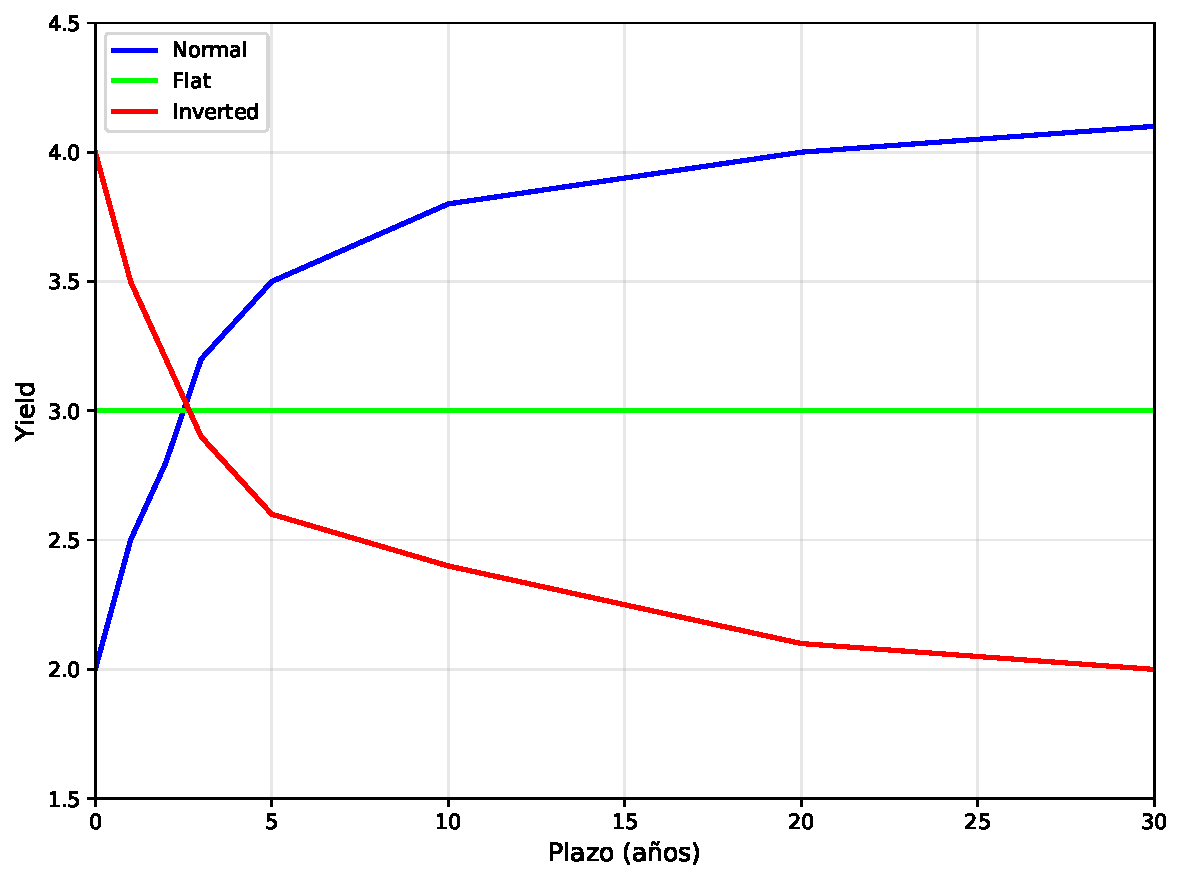
\includegraphics[width=0.65\linewidth]{Imagenes/Parte1/11_Prods_renta_fija/Yield_Curve.pdf}
    \caption{Yield Curve}
\end{figure}




\subsection{Duración}
Hay dos maneras de definir la duración de un bono:
\begin{itemize}
    \item \textbf{Duración modificada}: mide la sensibilidad del precio del bono ante pequeños cambios en la tasa de interés. P.e.\ si la duración es de 5.1, entonces un aumento  del 1\% del interés reduce el precio del bono un 5.1\%. Se calcula como:
    \[
        \boxed{D_{\text{mod}} =  -\frac{1}{B}\frac{\partial B}{\partial y}}
    \]
    \item \textbf{Duración Macaulay}: es el tiempo promedio ponderado hasta que se reciben los flujos del bono. P.e.\ si la duración es de 4.2, significa que, en promedio, el inversor recupera su dinero en 4.2 años. Se calcula como:
    \[
        \boxed{D_{\text{mac}} = (1+y)D_{\text{mod}} = -\frac{1+y}{B}\frac{\partial B}{\partial y}}
    \]
\end{itemize}

Las derivadas para el caso discreto y continuo son:
\begin{itemize}
    \item Caso discreto:
    \begin{align}\label{eq:derivadas_bono_discreto}
        B &= \frac{P}{(1+y)^T} + \sum_{t=1}^{T} \frac{C_t}{(1+y)^t} \notag \\
        \frac{\partial B}{\partial y} &= -\frac{P T}{(1+y)^{T+1}} - \sum_{t=1}^{T} \frac{C_t t}{(1+y)^{t+1}} = - \frac{1}{1+y}\left( \frac{P T}{(1+y)^{T}} + \sum_{t=1}^{T} \frac{C_t t}{(1+y)^{t}} \right) \\
        \frac{\partial^2 B}{\partial y^2} &= \frac{P T (T+1)}{(1+y)^{T+2}} + \sum_{t=1}^{T} \frac{C_t t (t+1)}{(1+y)^{t+2}} = \frac{1}{(1+y)^2}\left( \frac{P T (T+1)}{(1+y)^{T}} + \sum_{t=1}^{T} \frac{C_t t (t+1)}{(1+y)^{t}} \right)  \notag
    \end{align}
    \item Caso continuo:
    \begin{align}\label{eq:derivadas_bono_continuo}
        B &= P e^{-yT} + \sum_{t=1}^{T} C_t e^{-yt}  \notag \\
        \frac{\partial B}{\partial y} &= -P T e^{-yT} - \sum_{t=1}^{T} C_t t e^{-yt} \\
        \frac{\partial^2 B}{\partial y^2} &= P T^2 e^{-yT} + \sum_{t=1}^{T} C_t t^2 e^{-yt}  \notag
    \end{align}
\end{itemize}
por lo que las duraciones son:
\begin{itemize}
    \item Caso discreto:
    \begin{align*}
        D_{\text{mod}} &=  -\frac{1}{B}\frac{\partial B}{\partial y} = -\frac{1}{B}\left(- \frac{1}{1+y}\left( \frac{P T}{(1+y)^{T}} + \sum_{t=1}^{T} \frac{C_t t}{(1+y)^{t}} \right)\right) \\
        &= \boxed{ \frac{1}{1+y}\left( \frac{ \frac{P T}{(1+y)^{T}} + \sum_{t=1}^{T} \frac{C_t t}{(1+y)^{t}} }{ \frac{P}{(1+y)^T} +\sum_{t=1}^{T} \frac{C_t}{(1+y)^t} } \right) } \\
        D_{\text{mac}} &= \boxed{ (1+y)D_{\text{mod}} = \frac{ \frac{P T}{(1+y)^{T}} + \sum_{t=1}^{T} \frac{C_t t}{(1+y)^{t}} }{ \frac{P}{(1+y)^T} +\sum_{t=1}^{T} \frac{C_t}{(1+y)^t} } }
    \end{align*}
    \item Caso continuo:
    \begin{align*}
        D_{\text{mod}} &=  -\frac{1}{B}\frac{\partial B}{\partial y} = \boxed{ \frac{ P T e^{-yT} + \sum_{t=1}^{T} C_t t e^{-yt} }{ P e^{-yT} + \sum_{t=1}^{T} C_t e^{-yt} } } \\
        D_{\text{mac}} &= (1+y)D_{\text{mod}} = \boxed{ (1+y)\frac{ P T e^{-yT} + \sum_{t=1}^{T} C_t t e^{-yt} }{ P e^{-yT} + \sum_{t=1}^{T} C_t e^{-yt} } }
    \end{align*}
\end{itemize}




\subsection{Convexividad}
Es otro orden para medir la sensibilidad del precio del bono frente a cambios del interés. Una mayor convexidad implica menor pérdida ante subidas de tasas y mayor ganancia ante bajadas. Se calcula como:
\[
    \boxed{C = \frac{1}{B}\frac{\partial^2 B}{\partial y^2}}
\]
observando las derivadas calculadas en~\eqref{eq:derivadas_bono_discreto} y~\eqref{eq:derivadas_bono_continuo}tiene que:
\begin{itemize}
    \item Caso discreto:
    \[
        C = \frac{1}{B}\frac{\partial^2 B}{\partial y^2} = \boxed{ \frac{1}{(1+y)^2} \frac{ \frac{P T (T+1)}{(1+y)^{T}} + \sum_{t=1}^{T} \frac{C_t t (t+1)}{(1+y)^{t}} }{ \frac{P}{(1+y)^T} + \sum_{t=1}^{T} \frac{C_t}{(1+y)^t}}  }
    \]
    \item Caso continuo:
    \[
        C = \frac{1}{B}\frac{\partial^2 B}{\partial y^2} = \boxed{ \frac{P T^2 e^{-yT} + \sum_{t=1}^{T} C_t t^2 e^{-yt}}{P e^{-yT} + \sum_{t=1}^{T} C_t e^{-yt}} }
    \]
\end{itemize}






\subsection{Intereses dependientes del tiempo (Time-Dependent Interest Rates)}
Se considera un interés dependiente del tiempo $r(t)$, por lo que el valor del bono también es dependiente del tiempo $B(t)$. Se considera que el principal 1, por lo que $B(T)=1$. Todas las constantes que se calculan a continuación son relativas a esta condición.

Se tiene por una parte que la variación del valor del bono es:
\[
    \frac{dB}{dt} = \frac{dB}{dt} \Rightarrow dB = \frac{dB}{dt} dt
\]
este argumento se puede justificar de forma más estricta con intervalos infinitesimales o aproximaciones de Taylor. Para evitar arbitraje se iguala al interés:
\begin{align}\label{eq:interes_dependiente_tiempo}
    dB = \frac{dB}{dt} dt = r(t) B dt \Rightarrow B(t; T) = e^{\int_{t}^{T} r(\tau) d\tau}
\end{align}

Estudiando ahora el caso de un bono con cupones, se tiene que se ha recibido un cupón $K(t)dt$ en el periodo $[t, t+dt]$, por lo que la variación del valor del bono es:
\[
    dB = \left( \frac{dB}{dt} + K(t) \right) dt
\]
que igualando al interés:
\[
    \frac{dB}{dt} + K(t) = r(t) B \Rightarrow \boxed{B(t; T) = e^{\int_{t}^{T} r(\tau) d\tau} \left( 1 + \int_t^T K(t') e^{\int_{t}^{T} r(\tau) d\tau} dt' \right)}
\] 
habiendo elegido las constantes para que $B(T)=1$.







\subsection{Tasas Forward y bootstrapping}\label{sec:forward_bootstrapping}
Es la tasa de interés esperada de un bono sabiendo la tasa de interés actual de varios bonos de cupón cero con diferentes vencimientos. 

En el caso continuo, y que todo es diferenciable correctamente, no hace falta más que la ecuacion~\eqref{eq:interes_dependiente_tiempo} para calcular la tasa forward $f(t, T)$ entre dos fechas $t$ y $T$. 
\[
    Z(t; T) = e^{\int_{t}^{T} r(\tau) d\tau} \Rightarrow r(T) = -\frac{\partial}{\partial T} \left( \ln(Z(t;T)) \right) \Rightarrow F(t;T) = -\frac{\partial}{\partial T} \left( \ln(Z(t;T)) \right) 
\]
que en términos de rendimiento se tiene que
\[
    Z(t; T) = e^{-y(t;T)(T-t)} \Rightarrow \boxed{F(t;T) = y(t;T) + \frac{\partial y}{\partial T}}
\]



Para el caso discreto se consideran varios bonos de cupón cero ordenados según su vencimiento, siendo el primero el que tenga el vencimiento más temprano. Luego se tiene $Z_i^M$ siendo $i$ la posición en el ranking. EL primer bono tendrá tiene un interés implícito de
\[
    Z_1^M = e^{y_1(T_1-t)} \Rightarrow y_1 = \frac{\ln(Z_1^M)}{T_1-t}
\]
este es el interés que se usa para descontar desde el momento actual hasta  $T_1$ para todos los bonos e instrumentos. Por lo tanto el interés implícito del segundo bono sería
\[
    Z_2^M = e^{-y_1(T_1-t)} e^{y_2(T_2-T_1)} \Rightarrow y_2 = \frac{\ln(Z_2^M/Z_1^M)}{T_2-T_1}
\]
se puede seguir este proceso de forma iterativa para los bonos que hagan falta. A esto se le llama \textbf{bootstrapping}.







